\section{Versuchsaufbau und Versuchsdurchführung}

\begin{flushleft}
    Für diesen Versuch wird eine Hochvakuumdiode, zwei regelbare Konstantspannungsgeräte, eine regelbares Konstantspannungsgeräte, welches eine Spannung von $0\,\unit{\volt}$ bis $1\,\unit{\volt}$ generiert, Kabel und ein viel kürzeres und dünneres Kabel verwendet.
    Zusehen sind diese Sachen in der Abbildung \ref{Abbildung3}. 
\end{flushleft}

\begin{figure}[H]
    \centering
    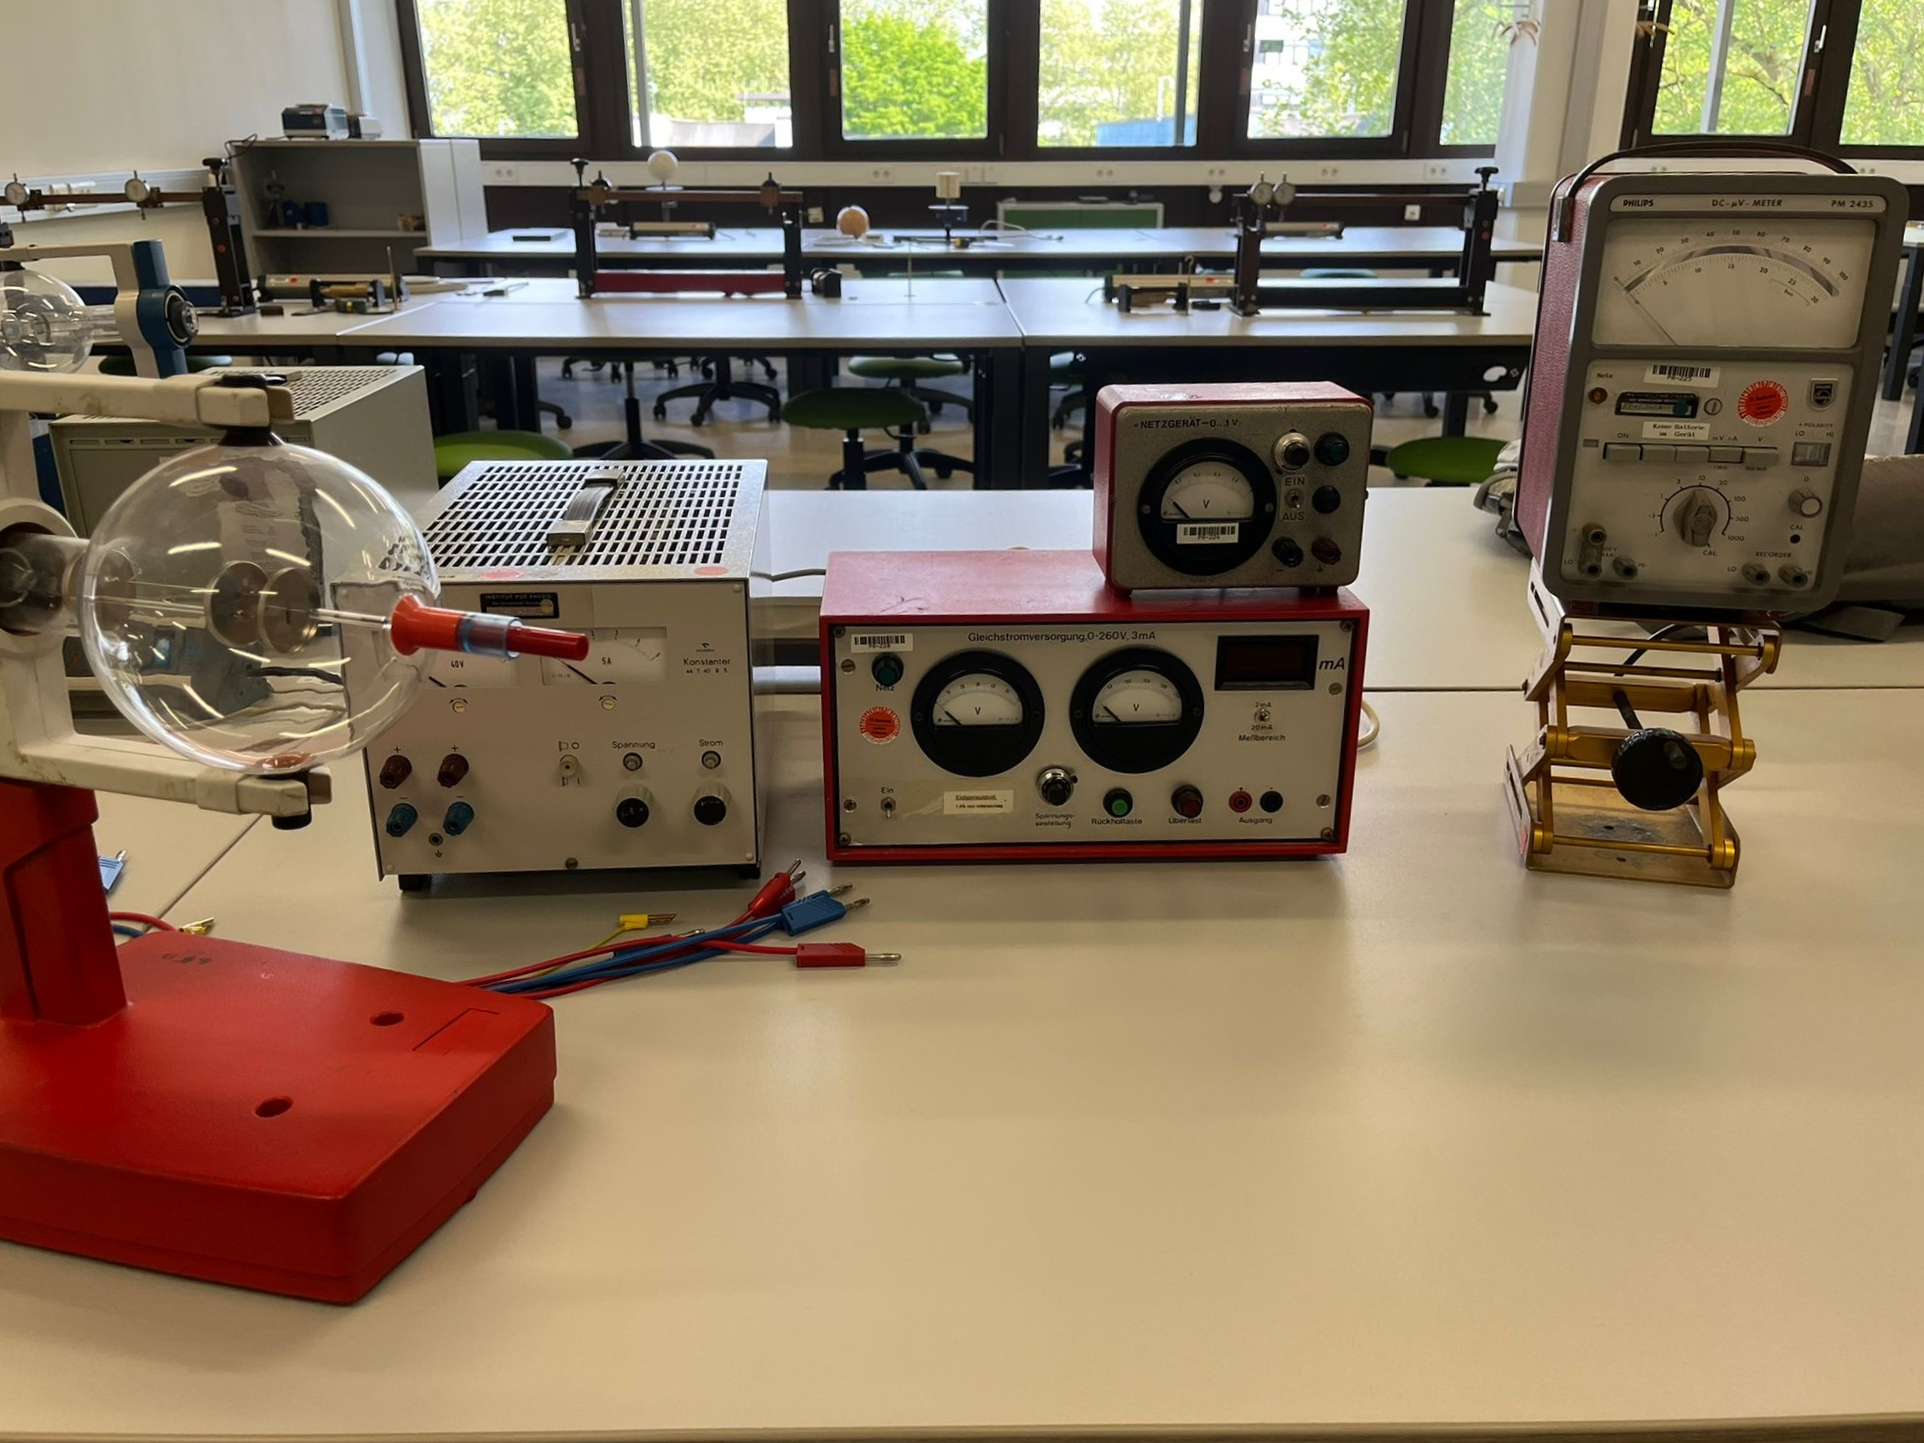
\includegraphics[height=70mm]{bilder/V1.jpeg}
    \caption{Verbildlichung aller verwendeten Materialien. \label{Abbildung3} }
\end{figure}

\subsection{Kennlinienschar einer Hochvakuumdiode }

\begin{flushleft}
    Für den ersten Versuchsteil wird die Schaltung, wie Abbildung \ref{Abbildung4} zu sehen, aufgebaut.
    Danach werden beide Spannungsgeräte angeschaltet und der Strom des oben links, in Abbildung \ref{Abbildung4}, abgebildeten Spannungsgeräts auf $2\,\unit{\ampere}$ gestellt und der Spannungswert aufgenommen.
    Als nächstes werden die Spannung und der Strom des Gleichstromversorgers aufgenommen.
    Dies wird für die Anodenströme von $2,0\,\unit{\ampere} - 2,5\,\unit{\ampere}$ jeweils aufgenommen. 
\end{flushleft}

\begin{figure}[H]
    \centering
    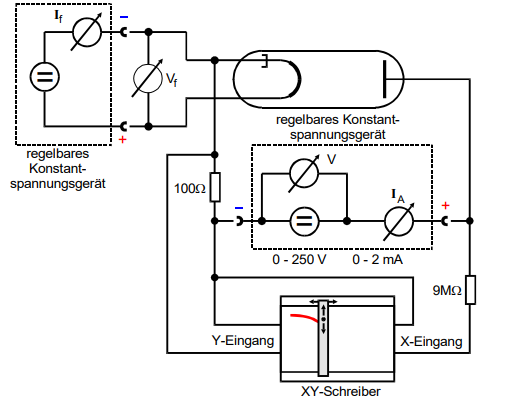
\includegraphics[height=70mm]{bilder/V2.png}
    \caption{Schaltung zur Aufnahme von Diodenkennlinien \cite{a1}. \label{Abbildung4} }
\end{figure}

\subsection{Maximal mögliche Heizleistung}

\begin{flushleft}
    Als nächstes wird die Schaltung, wie in Abbildung \ref{Abbildung5} zu sehen, umgebaut.
    Der Heizstrom wird auf $2,5\,\unit{\ampere}$ gestellt.
    Die Gegenspannung wird in einem Bereich von $0\,\unit{\ampere}$ bis $1\,\unit{\ampere}$ in $0,1$ Schritte variiert und der daraus resultierende Strom aufgenommen. 
\end{flushleft}

\begin{figure}[H]
    \centering
    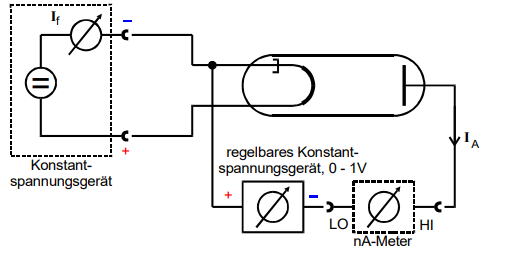
\includegraphics[height=50mm]{bilder/V3.png}
    \caption{ Schaltung zur Aufnahme einer Anlaufstromkurve \cite{a1}. \label{Abbildung5} }
\end{figure}